\section{Inquadramento territoriale}

Il lago di Endine si trova nell'alta Val Cavallina, dove si è formato nell'epoca quaternaria in seguito ai movimenti di escavazione dovuti al movimento delle masse glaciali. Il lago è classificato come lago glaciale vallivo. Confrontato con altri laghi di origine glaciale, è caratterizzato da una profondità media relativamente bassa.
La scarsa profondità ha giocato un ruolo fondamentale nei processi di degrado ambientale e successivo recupero, che ha interessato il lago negli ultimi 50 anni. 

Il bacino lacustre presenta la conformazione tipica dei laghi di origine glaciale: ha una forma allungata secondo l’andamento della valle che occupa la parte centrale, donandole caratteristiche peculiari tra cui una variegata flora spontanea. 
Con una forma allungata, lungo l’asse nord-est, sud-ovest. Il lago è situato a 340 metri di altitudine ed è alimentato da numerosi torrenti che scendono dai monti circostanti e ha un unico emissario, il Cherio, che scorre poi nella pianura per poi confluire nell'Oglio.

Sulle sponde del lago si affacciano quattro comuni: Spinone, Ranzanico, Endine Gaiano e Bianzano.

\begin{figure}[H]
	\centering
	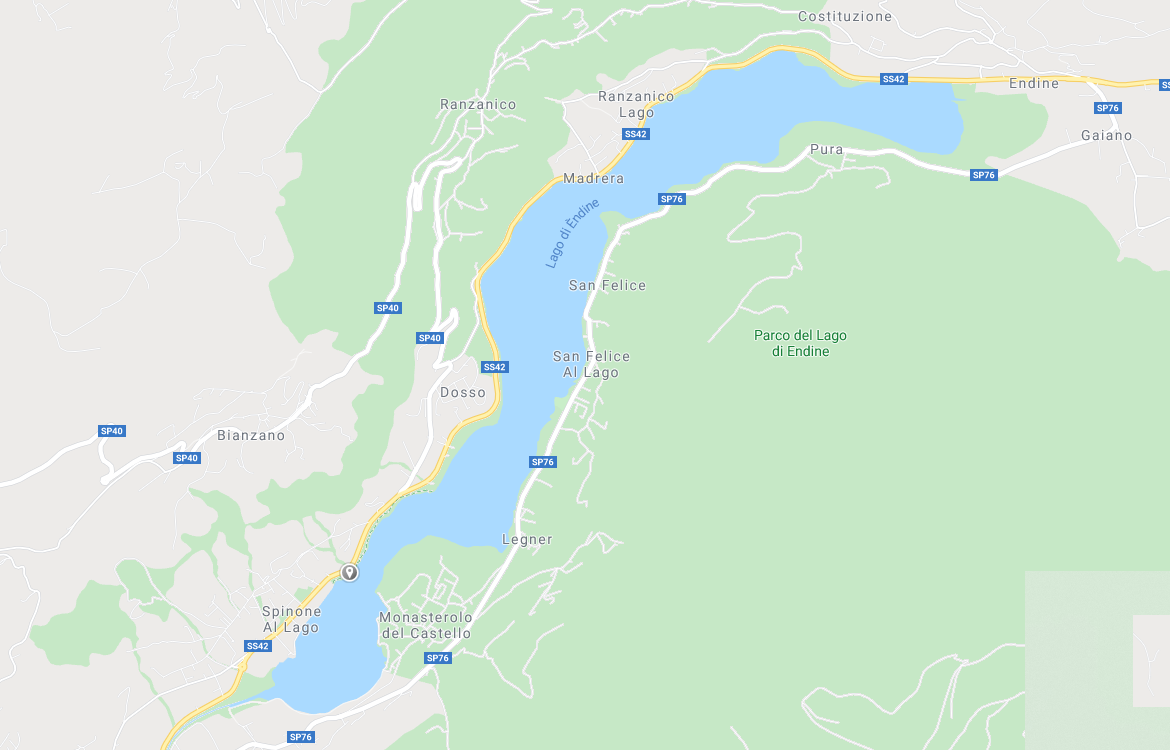
\includegraphics[width=0.6\textwidth]{image12}
	\caption{Mappa}
	\label{fig:mesh1}
\end{figure}

Il lago, incassato nella stretta valle tra alti rilievi, ha conservato pressoché intatto l'ambiente naturale; classificato in un primo tempo come zona di rilevante interesse ambientale dalla Regione Lombardia; successivamente come parco e come tale soggetto a tutela. Le rive alternano fitti canneti, che sono luogo di riproduzione della ricca fauna ittica e rifugio per la fauna avicola, a piccole spiagge molto frequentate nei fine settimana da turisti che vi possono consumare la colazione al sacco in aree appositamente attrezzate; ma anche vi si può praticare  sport d'acqua, tra cui: vela, windsurf, canoa, canottaggio ed infine la pesca.

\begin{figure}[H]
	\captionsetup[subfloat]{farskip=2pt,captionskip=8pt}
	\centering
	\subfloat[M. Girone]{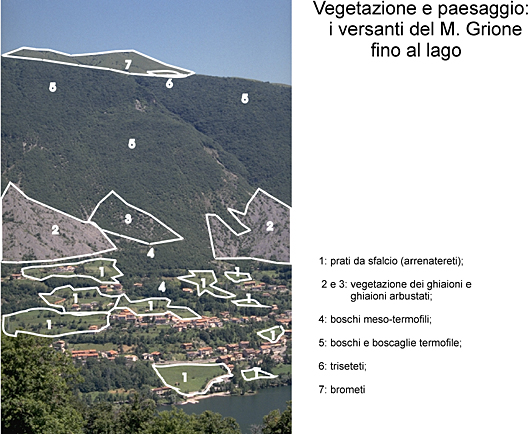
\includegraphics[width=6cm]{image40}}
	\hspace{1cm}
	\subfloat[Valle del torrezzo]{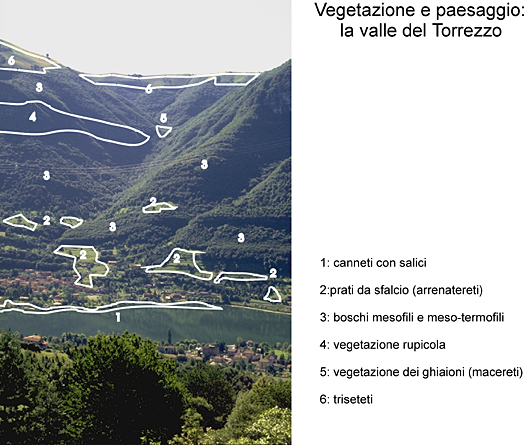
\includegraphics[width=6cm]{image5}}
	\caption{Vegetazione e paesaggio}
	\label{fig:fotolago}
\end{figure}

\begin{figure}[H]
	\centering
	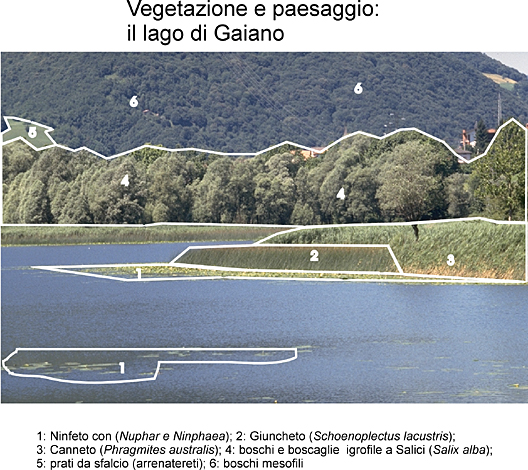
\includegraphics[width=0.4\textwidth]{image2}
	\caption{Lago di Gaiano}
	\label{fig:mesh1}
\end{figure}




Nella \cref{fig:fotolago} possiamo vedere delle fotografie raffiguranti il lago. Notiamo nel dettaglio 3 viste in cui possiamo \todo{finisci qua}

\begin{wrapfigure}[9]{r}{0.5\textwidth}
	\centering
	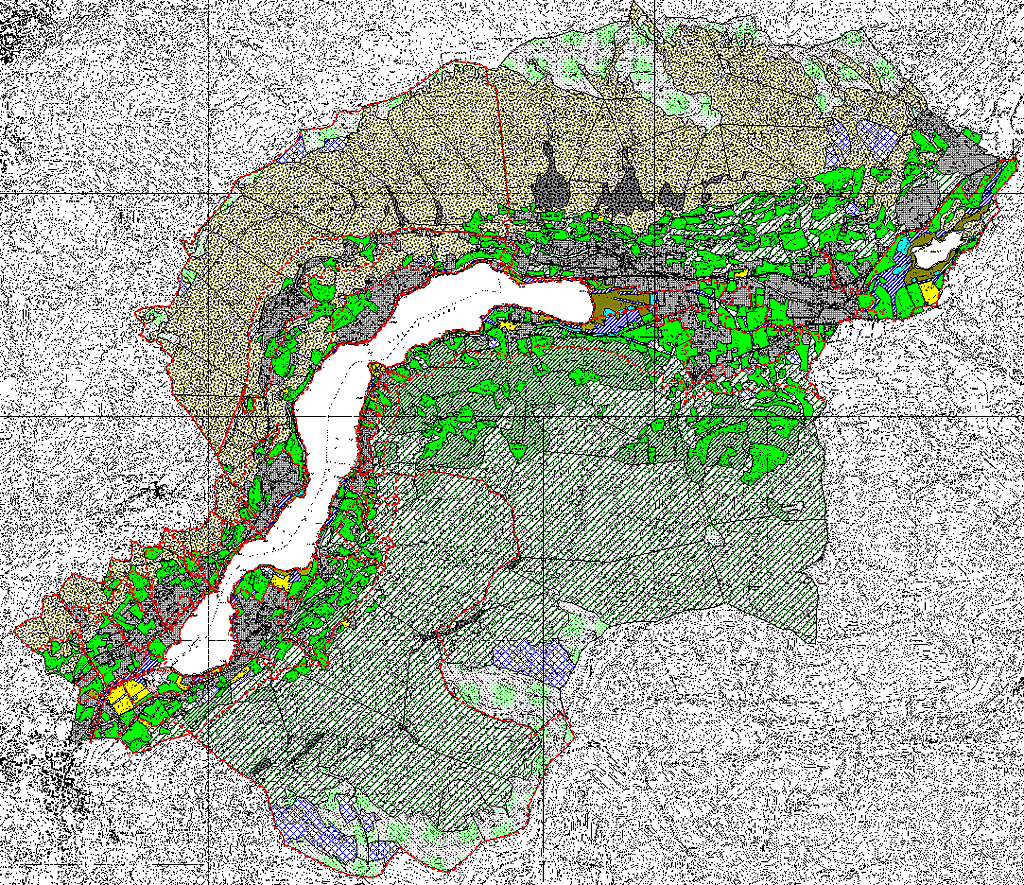
\includegraphics[width=0.4\textwidth]{image44}
	\caption{Mappa}
\end{wrapfigure}

Le acque, sufficientemente limpide, tendono ad un caratteristico colore verde scuro.
Il perimetro del lago è totalmente percorribile.

\subsection{Vegetazione autoctona}




L'area dei laghi di Endine si contraddistingue per la presenza di formazioni igrofile e palustri. Verso le rive sono presenti fasce di ninfeti costituiti da Ninfa e Ninfa gialla, cui sono associate altre specie tra cui il Ranuncolo d’acqua.

\begin{wrapfigure}[23]{r}{0.5\textwidth}
	\centering
	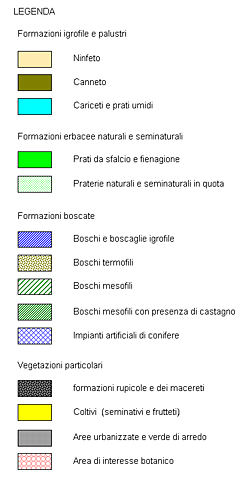
\includegraphics[width=0.4\textwidth]{image18}
	\caption{Legenda}
\end{wrapfigure}

Il lago è circondato da una fascia quasi continua di canneto, in cui abbondano sequenze costituite da Cannuccia di palude seguita da Scirpo, in posizione più esterne, e da Tifae, localizzata sulle rive. 

Ai margini delle aree lacustri, o lungo alcuni piccoli immissari, sono presenti formazioni boscate igrofile nelle quali si possono osservare Ontani neri, Frassini maggiori, Pioppi neri, Salici bianchi e raramente Platani. Nello strato arbustivo si segnala la presenza di Sanguinella, Sambuco, Aglio orsino, Rovi, Oppio, Ortica mora e Canapa acquatica.  Nei siti più vicini all'acqua sono osservabili anche Noccioli, Biancospini , Salici, Ontani neri, Frangola e Dulcamara. Sui versanti meno soleggiati sono presenti formazioni boscate mesofile, costituite da specie quali aceri di monte, Frassini maggiori, Carpini bianchi , Ciliegi selvatici, Conifere, Castagneti e Faggi ad alte quote.  Sui fianchi ben assolati e meglio esposti attorno al lago sono insediate formazioni boscate termofile dove si osservano Carpini neri, Roverelle e Ornielli.

\pagebreak